%!TEX root = ../thesis.tex

\chapter{Implementierung und Evaluation} % (fold)
\label{cha:implementierung_und_evaluation}

\todo[inline]{Auf die verschiedenen Klassen von Facebook und Co eingehen, REST, SOAP, OAUTH, Client/Passwort, Art der Plattforn, Forum, OSN, Videoplatform}

\section{Verwendete Programme und Bibliotheken} % (fold)
\label{sec:verwendete_bibliotheken_und_programme}

An dieser Stelle soll noch kurz auf zusätzliche Programm und Bibliotheken eingegangen werden, die für die Entwicklung der einzelnen Connectoren hilfreich waren. 

\subsection{Apache Maven} % (fold)
\label{sub:apache_maven}

Für die Entwicklung der Programme und Bibliotheken dieser Arbeit wurde das Buil-Management Programm \texttt{Maven}\footnote{http://maven.apache.org/} von Apache eingesetzt. Mit diesem ist es auf einfache Art möglich Java-Programme zu verwalten und zu erstellen. So ist nur mit einer einzigen XML-Datei (\texttt{pom.xml}) die Abhängigkeiten festzulegen, das Programm zu kompilieren, zu testen und es auszuliefern. Maven schreibt eine feste Ordnerstruktur für ein Projekt vor wie der Produktivquellcode, dafür nötige Ressource (Bilder, Teste,\dots) und der Code zum Testen geordnet werden sollen. Die Abhängigkeiten werden automatisch aus zentralen Repositories heruntergeladen und ins Projekt eingebunden. So muss dies nicht immer von Handgeschehen und spart so Arbeit.

% subsection apache_maven (end)

\subsection{RDF2Go} % (fold)
\label{sub:rdf2go}

% subsection rdf2go (end)

% section verwendete_bibliotheken_und_programme (end)

\section{Implementierung der Connectoren} % (fold)
\label{sec:implementierung_der_connectoren}

An dieser Stelle soll beschrieben werden wie Connectoren für die in Abschnitt \ref{sec:lernplattformen_und_soziale_online_netzwerke} vorgestellten Plattformen implementiert werden können. Dafür wird darauf eingegangen mit welcher Art von API auf die Daten der einzelnen Plattformen zugegriffen werden und wie man deren Datenstruktur in SIOC abbilden kann. Ebenfalls werden auftretende Probleme und wenn möglich deren Lösung gezeigt.

\subsection{Allgemeine Informationen zum Mapping nach SIOC} % (fold)
\label{sub:allgemeine_informationen_zum_mapping_nach_sioc}

Innerhalb der Beschreibungen des Mappings nach SIOC werden zur besseren Übersicht und einfacheren Lesbarkeit Platzhalt für einige URIs benutzt. Welche Platzhalten dies sind und für welche URI sie stehen ist aus Tabelle \ref{tbl:platzhalter_fuer_sioc_mapping} zu entnehmen.
\begin{table}[ht]
    \centering
    \caption{Allgemeine Platzhalter und deren Beschreibung für das Mapping nach SIOC}
    \begin{tabular}{l|p{11cm}}
        \textbf{Platzhalter} & \textbf{Bedeutung} \\ 
        \hline
        \texttt{\{rootUri\}} & Die WurzelUri einer SOC. Für Facebook wäre dies zum Beispiel \texttt{https://www.facebook.com} \\
        \texttt{\{siteUri\}} & URI für eine SIOC Site \\
        \texttt{\{serviceUri\}} & URI für einen SIOC Service \\
        \texttt{\{userAccountUri\}} & URI für einen SIOC UserAccount \\
        \texttt{\{forumUri\}} & URI für ein SIOC Forum \\
        \texttt{\{threadUri\}} & URI für ein SIOC Thread \\
        \texttt{\{postUri\}} & URI für ein SIOC Post
    \end{tabular}
    \label{tbl:platzhalter_fuer_sioc_mapping}
\end{table}

Da einige Eigenschaften der Klassen von SIOC bei allen Plattformen mit ähnlichen Werten belegt werden und sich nur vom Aufruf der API unterscheiden, sollen zuvor für die Klassen UserAccount, Forum, Thread und Post die Eigenschaften beschrieben werden, die überall verwendet werden.

\begin{description}
    \item[\textbf{UserAccount:}]  Für die Klasse UserAccount ist die Angabe von vier Eigenschaften wichtig. Die erste ist \texttt{sioc:Id} mit der die ID des Benutzerkontos angegeben wird und \texttt{sioc:name} für den den Benutzernamen. Aus Kompatibilitätsgründen mit FOAF wird die ID des Benutzers noch mit \texttt{foaf:accountName} angegeben und die URI zum verwendeten Service mit \texttt{foaf:accountServiceHomepage}. Die Angabe der Daten zu Autorisierung erfolgt mit der Eigenschaft \texttt{siocsa:accountAuthentication}.

    \item[\textbf{Forum:}] Jedes Forum hat seine eigene ID, die wie bei UserAccount unter der Eigenschaft \texttt{sioc:id} abgelegt wird. Ebenfalls bekommt jedes Forum einen Namen mit \texttt{sioc:name}. Jedes Forum hat eine Site von der es gehostet wird (\texttt{sioc:has\_host}). Ein Forum dient als Container für Post, die mit der Eigenschaft \texttt{sioc:container\_of} gekennzeichnet werden. Zugleich kann es auch Threads mit \texttt{sioc:parent\_of} enthalten. 

    \item[\textbf{Thread:}] Ein Thread enthält ebenfalls wieder eine ID und einen Namen. Enthält nur Beiträger der Klasse Post mit \texttt{sioc:container\_of} und ist immer ein Teil eines Forums mit \texttt{sioc:has\_parent}.

    \item[\textbf{Post:}] Jeder Post hat eine, für die Seite eindeutige ID mit \texttt{sioc:id}. Mit der Eigenschaft \texttt{sioc:creator} wird der UserAccount des Autors festgelegt und mit \texttt{sioc:content} der Inhalt des Beitrags. Besitzt ein Beitrag eine Titel, wird dieser mit \texttt{sioc:title} gespeichert. Der Zeitpunkt der Erstellung kommt nach \texttt{dcterms:created} und der bei eine Modifikation nach \texttt{dcterms:modified}. Beiträge gehören immer zu einen Forum oder Thread welches mit \texttt{sioc:has\_container} angegeben wird. Auch können Beiträge Kommentare mit \texttt{sioc:has\_reply} enthalten oder selber Kommentare auf andere Beiträge mit \texttt{sioc:reply\_of} sein.
\end{description}

% subsection allgemeine_informationen_zum_mapping_nach_sioc (end)

\subsection{Allgemeine Probleme und Lösungen bei der Implementierung} % (fold)
\label{sub:allgemeine_probleme}

Bei der Implementierung der Connectoren treten ab und zu Probleme auf, die unabhängig von der verwendeten API gelöst werden müssen. Hier sollen diese Probleme und deren Lösung beschrieben werden. 

\subsubsection{Doppelte Beiträge beim Synchronisieren} % (fold)
\label{ssub:doppelte_beitraege_beim_synchronisieren}

Sollen zwei Threads auf unterschiedlichen Plattformen synchronisiert werden, tritt automatisch das Problem auf, dass Beiträge die von A nach B geschrieben wurden beim auslesen von B wieder bei A als \enquote{neuer} Beitrag landen würde, obwohl er ursprünglich von dort kam. Dies würde ohne Eingreifen zu einer Dauerschleife führen, bei der die selben Beiträge immer hin und her geschrieben werden. 

Aus diesem Grund wird vor dem Schreiben eines Beitrags eine Art Wasserzeichen an diesen Angebracht. Diese Wasserzeichen besteht aus der Zeichenkette \texttt{--- forwarded by SOCC {siteUri} ---}. Hierzu muss jedem Beitrag mit der Eigenschaft \texttt{dcterms:isPartOf} die URI des Site Objekts zu dem der Beitrag gehört, hinzugefügt werden. Wird nun eine Beitrag gelesen, der ursprünglich von der Site des Connectors kam, wird dieser ignoriert. Enthält dagegen der Beitrag schon eine Wasserzeichen mit der URI einer anderen Site, wird kein neues Wasserzeichen hinzugefügt.

% subsubsection synchronisieren_von_beitrage (end)

\subsubsection{Rekonstruktion der Kommentarstruktur} % (fold)
\label{ssub:rekonstruktion_der_kommentarstruktur}

Bei der Synchronisation ist es ebenso wichtig die Struktur von Kommentaren beizubehalten. Wenn Beitrag A2 ein Kommantar auf Beitrag A1 auf Seite A muss diese Struktur beim Synchronisieren mit Seite B mit den Beiträgen B1 und B2 erhalten bleiben.

\begin{figure}[ht]
    \centering
    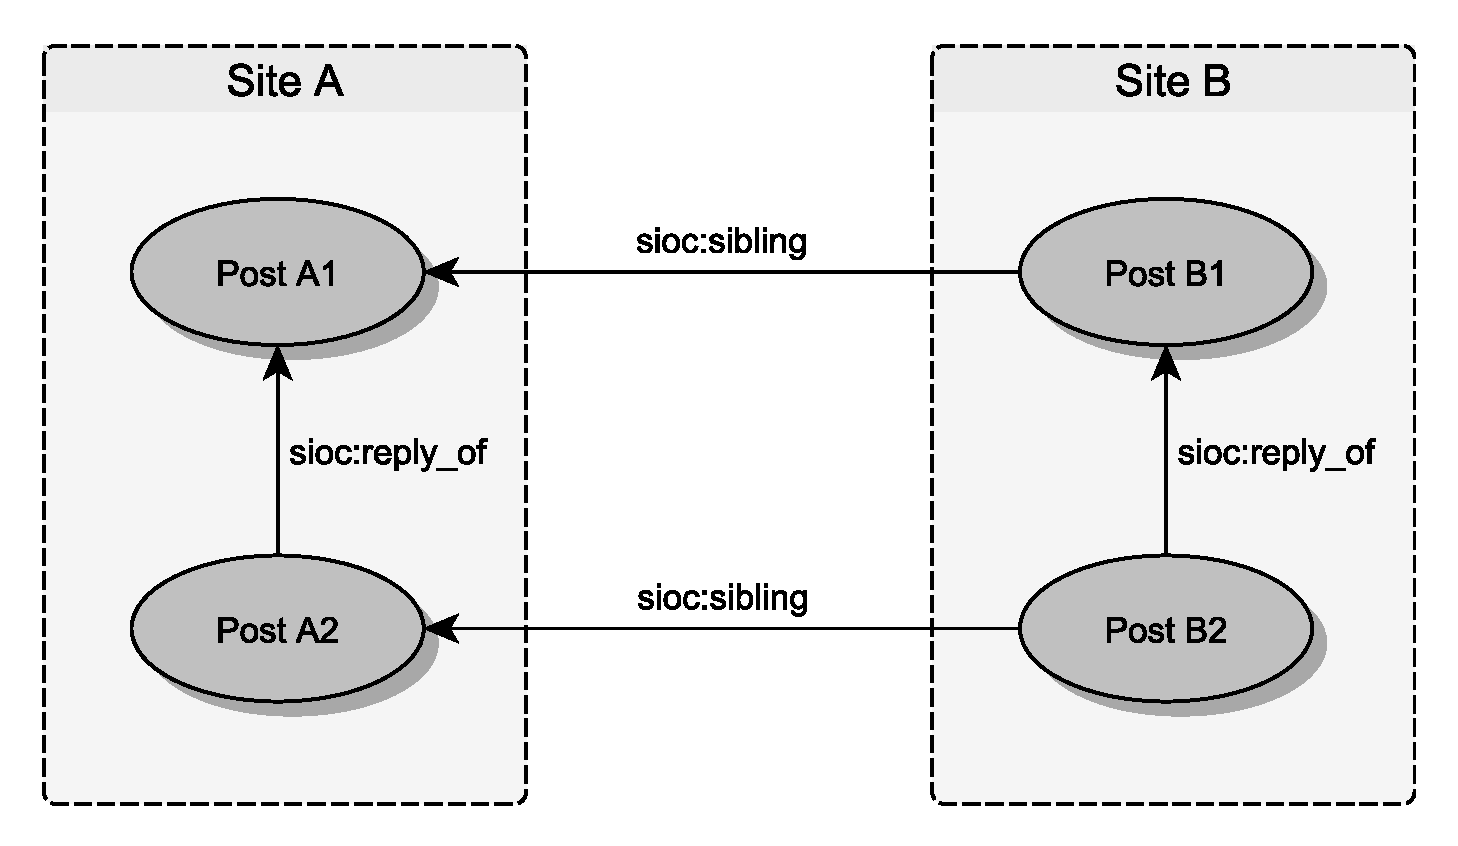
\includegraphics[
        width=0.7\textwidth,
        keepaspectratio=true
    ]{assets/images/comment_structuring}
    \caption{Erhalten der Kommentarstruktur beim Schreiben von Beiträgen}
    \label{fig:kommentarsturktur_beim_schreiben}
\end{figure}

Hierzu wird nach dem Schreiben eines Beitrags mit der Eigenschaft \texttt{sioc:sibling} (Englisch für Geschwister) die URI zum original Beitrag beim geschriebenen Beitrag festgehalten. Taucht nun beim Schreiben ein Beitrag auf, der ein Kommentar auf den mit \texttt{sioc:sibling} gespeicherten Beitrags ist, kann dieser an die richtige Stelle als Kommentar geschrieben werden. Der RDF-Graph nach dem Synchronisieren ist in Abbildung zu sehen. 

% subsubsection rekonstruktion_der_kommentarstruktur (end)

% subsection allgemeine_probleme (end)

\subsection{Moodle Connector} % (fold)
\label{sub:moodle_connector}

% \begin{itemize}
%     \item Eingebaute REST Schnittstelle, aber kein Lesen von Beiträgen
%     \item WebService Plugin MoodleWS (REST oder SOAP)
%     \begin{itemize}
%         \item https://github.com/patrickpollet/moodlews
%         \item ClientAPI existieren von selber Autor
%         \item REST defekt, kein schreiben von Beiträgen möglich
%         \item SOAP funktioniert mehr oder weniger
%         \item Verschluckt Fehlermeldungen
%         \item kein lesen einzelner Posts/Threads/Foren
%         \item SOAP ClientAPI neu generieren, weil vorhandene nicht mit 2.4 funktioniert.
%         \item Username/Password + Session Token/Id
%         \item “Use an auto generated wsdl” -> No
%         \item schreiben von neuen Beitrag direkt in thread nur als Antwort auf ersten Beitrag möglich
%         \item Rückgabe aller Beiträge in einem Objekt
%     \end{itemize}
% \end{itemize}

\subsubsection{Moodle Webservice API} % (fold)
\label{ssub:moodle_webservice}

Moodle bringt von Haus aus schon eine Webservice-Schnittstelle für einen Zugriff auf seine Daten mit. Diese API unterstützt dabei Protokolle für REST, SOAP und oder XML-RPC\footnote{\url{http://xmlrpc.scripting.com/}}. Mit ihr können Kurse, Foren und deren Threads (in Moodle Discussion Topics genannt), Benutzerprofile, Gruppen und viele andere Ressourcen ausgelesen oder geschrieben werden. Leider gilt dies nicht für Beiträge innerhalb von Foren Threads. Die aktuelle Version (Beim verfassen dieser Arbeit war dies 2.5.1) erlaubt es nicht Beiträge weder zu lesen noch zu schreiben.

Doch existiert ein Plugin für Moodle, dass auf dieser Webservice API aufbaut und erweitert - \emph{MoodleWS}\footnote{\url{https://github.com/patrickpollet/moodlews}}. MoodleWS bietet den Zugriff über REST und SOAP, wobei bei der Verwendung von REST JSON als Datenformat verwendet wird und nicht XML wie mit SOAP. Mit diesem Plugin ist ein Programm nun auch in der Lage Beiträge aus Threads zu lesen. Die REST-Schnittstelle hat aber noch eine paar Fehler und so können damit noch keine neuen Beiträge geschrieben werden. Mit SOAP ist dies aber problemlos möglich.

Für die Benutzung der muss sich ein Client mit dem Benutzernamen und Passwort eines vorhandenen Benutzers anmelden. Ist dies erfolgreich, bekommt der Client einen zufällig ID und einen Sitzungsschlüssel die er bei jeder Abfrage angeben muss. Dieser Sitzungsschlüssel ist nur eine begrenzte Zeit gültig, so kann es passieren, dass eine Operation fehlschlägt und der Client sich neu anmelden muss.

Für die Verwendung der API in Java wird auch eine Bibliothek moodle\_ksoap2\footnote{\url{https://github.com/patrickpollet/moodlews\_ksoap2}} zur Verfügung gestellt. Sie abstrahiert komplett das SOAP-Protokoll im Hintergrund und enthält für alle Moodle-Ressource Java-Klassen und Methoden für den Zugriff. Bevor moodlews\_ksoap2 benutzt werden kann, ist darauf zu achten in Moodle unter \enquote{Site administration}, \enquote{Development}, \enquote {OK Tech Webservices ( aka wspp)} die Einstellung \enquote{Use an auto generated wsdl} auszuschalten, da es sonst zu Problemen mit moodlws\_ksoap2 kommen kann.

\begin{lstlisting}[
    caption={MoodleWS mit moodlews\_ksoap2: Lesebeispiel}\label{lst:moodlews_java_beispiel},
    captionpos=t]
Mdl_soapserverBindingStub client = new Mdl_soapserverBindingStub(
        MOODLE_URI + "/wspp/service_pp2.php",
        MOODLE_URI + "/wspp/wsdl2",
        false );

LoginReturn loginReturn = client.login(username, password);

ForumRecord[] forumRecords = client.get_all_forums(
        loginReturn.getClient(),
        loginReturn.getSessionKey(),
        "",
        "" );

for(ForumRecord forum : forumRecords){
    System.out.println(forum.getId() + " " + Forum.getName());
}
\end{lstlisting}

Wie in der ersten Zeile von Listing \ref{lst:moodlews_java_beispiel} zu sehen wird als ist der Client eine Objekt der Klasse \texttt{Mdl\_soapserverBindingStub} aus moodlews\_ksoap2. Dem Konstruktor wird die URI auf die Datei \enquote{service\_pp2.php} (Zeile 3) und der XML-Namespace der WSDL-Datei des MoodleWS-Plugins übergeben. Das dritte Argument besagt, ob der Client im Debugmodus laufen und mehr Logging-Ausgaben macht über die einzelnen internen Abläufe ausgeben soll. In Zeile 6 meldet sich der Client mit einen Benutzernamen und einem Passwort bei MoodleWS an und bekommt ein Objekt der Klasse \texttt{LoginResult} mit der oben angesprochenen ID für den Client und einen Sitzungsschlüssel zurück. Mit der Methode \texttt{get\_all\_forums(\dots)} können nun ein Array mit allen Foren angefordert werden, auf die der angemeldete Benutzer Zugriff hat. Die ersten zwei Argumente dieser Methode sind die ID des Clients und der Sitzungsschlüssel. Mit den letzten zwei Argumenten kann das Ergebnis gefiltert werden. Dazu wird als erstes ein Spaltenname aus der Foren-Tabelle der Moodle-Datenbank angeben und als zweites welcher Wert dieser haben soll. Am Ende werden dann alle Ergebnisse mit der ID und Name des Forums ausgegeben.

\begin{lstlisting}[
    caption={MoodleWS mit moodlews\_ksoap2: Beitrag schreiben}\label{lst:moodlews_beitrag schreiben},
    captionpos=t]
ForumPostDatum postDatum = new ForumPostDatum(client
                    .getBindingStub()
                    .getNAMESPACE());

postDatum.setMessage("War kam bei der Aufgabe raus?");
postDatum.setSubject("Aufgabe 2.1");

client.forum_add_reply(
        client.getAuthClient(),
        client.getSessionKey(),
        postId,
        postDatum);
\end{lstlisting}

Beiträge können nur als Kommentare geschrieben werden und dessen ID bekannt sein. Alle Daten für den Beitrag werden in einem Objekt der Klasse \texttt{ForumPostDatum} gespeichert, wie in der ersten Zeile des Listings \ref{lst:moodlews_beitrag schreiben} zu sehen ist. Das Argument ist der beim Client angegebene XML-Namespace der WDSL-Datei. Als Daten können wie in Zeile 5 und 6 nur eine Nachricht (Message) und ein Thema (Subject) übergeben werden. Dieses Objekt wird dann an die Methode \texttt{forum\_add\_reply} mit der ID des Clients, dem Sitzungsschlüssel und der ID des Beitrags wohin geschrieben werden soll übergeben und an Moodle übertragen.s

% subsubsection moodle_webservice (end)

\subsubsection{Moodle Mapping nach SIOC} % (fold)
\label{ssub:moodle_mapping_nach_sioc}

Da Beiträge in Moodle in einer Forumsstruktur geschrieben werden, ist das Mapping nach SIOC problemlos möglich. Die Struktur von Moodle besteht aus der Klasse \texttt{Forum} und kann der gleich lautenden Klasse aus SIOC zugeordnet werden. Jedes Moodle Forum besteht aus einzelnen Objekten der Klasse \texttt{ForumDiscussions} welche der Klasse Thread aus SIOC entsprechen. Letztendlich werden die Beiträge mit der Klasse \texttt{ForumPost} aus Moodle modelliert, welche der Klasse Post aus SIOC zugeordnet werden kann. 

Die Tabelle \ref{tbl:moodle_sioc_uris} zeigt das Format der URIs, mit denen die Objekte der SIOC-Klassen in RDF benannt werden.

\begin{table}[ht]
    \centering
    \caption{URI Format für SIOC-Objekte aus Moodle }
    \begin{tabular}{l|p{11cm}}
        \textbf{SIOC Klasse} & \textbf{URI-Format} \\ 
        \hline
        Site & \texttt{\{rootUri\}}\\
        Service & \texttt{\{rootUri\}/wspp}\\
        UserAccount & \texttt{\{rootUri\}/user/profile.php?id=\{userId\}} \\
        Forum & \texttt{\{rootUri\}/mod/forum/view.php?id=\{forumId\}} \\
        Thread & \texttt{\{rootUri\}/mod/forum/discuss.php?d=\{discussionId\}} \\
        Post & \texttt{\{rootUri\}/mod/forum/discuss.php?d=\{discussionId\}\#p\{postId\}} \\
    \end{tabular}
    \label{tbl:moodle_sioc_uris}
\end{table}

% subsubsection moodle_mapping_nach_sioc (end)

\subsubsection{Besonderheiten bei der Implementierung des MoodleConnectors} % (fold)
\label{ssub:herausforderungen_bei_der_implementierung_des_moodleconnectors}

Der Connector für Moodle war wohl einer der herausforderndsten bei der Implementieren von allen fünf Connectoren. Nicht nur weil erst nach mehreren Test sich herausstellte, dass die favorisierte REST-Schnittstelle von MoodleWS kein schreiben von Beiträgen möglich macht sondern dass auch die Java-Bibliothek moodlews\_ksoap2 so ihre kleinen Eigenheiten hat. 

Zuerst mussten die Klasse für moodlews\_ksoap2 komplett neu generiert werden. In der Dokumentation wird beschrieben, dass dieser Schritt nötig ist, wenn sich an der WSDL-Datei von MoodleWS was geändert hat. Der passende Generator wird vom Entwickler gleich mitgeliefert und ist mit dem folgenden Befehl schnell bewerkstelligt.

\begin{lstlisting}[
    caption={Neugenerierung von moodlews\_ksoap2}\label{lst:neugenerierung_moodlews_ksoap2},
    captionpos=t]
    java  org.ksoap2.wsdl.WSDL2ksoap -p de.m0ep.moodlews.soap -o /tmp http://localhost/moodle/wspp/wsdl_pp2.php
\end{lstlisting}

Mit dem Parameter \enquote{-p} wir das Java-Package für die Java-Klassen festgelegt und mit \enquote{-o} der Ordner in dem die Klassen geschrieben werden. Die URI am Ende gibt den Pfad zur Datei \enquote{wsdl\_pp2.php} vom MoodleWS-Plugin. Diese ist dann an die jeweilige Moodleinstanz anzupassen.

Eine sehr nervende Eigenheit von moodlews\_ksoap2 ist die Tatsache, dass Java-Exceptions und Gründe für Fehler gerne verschluckt und nicht weitergegeben werden. So ist es zum Beispiel nicht möglich zu wissen ob eine Operation aufgrund eines Netzwerkfehlers, eines abgelaufenen Sitzungsschlüssels oder falschen Daten fehlschlug. Aus diesem Grund wurde der Client von moodlews\_ksoap2 für den ClientManager (siehe Abschnitt \ref{sub:clientmanager}) in eine extra Klasse \texttt{Moodle2ClientWrapper} gepackt und um Mechanismen zur Fehlererkennung und Wiederherstellung erweitert. Alle Funktionsaufrufe des Clients wie \texttt{get\_all\_forums(\dots)} werden dazu zuerst in die Methode \texttt{call} eines Objekts des Java-Interfaces \texttt{Callable<V>} verpackt, so dass diese Funktion, ohne zu wissen um welche es sich genau handelt, mehrfach aufrufen werden kann. Diese Objekt wird dann an die Methode \texttt{callMethod(\dots)} der Klasse \texttt{Moodle2ClientWrapper} übergeben. Diese Methode ruft dann zuerst die \texttt{call()} Methode des Callabel-Objekts und prüft ob ein gültiges Ergebnis zurückgegeben wurde. Dies ist der Fall wenn es ungleich \texttt{null} ist. Ist dies nicht der Fall, wird geschaut ob die Moodleinstanz erreichbar ist. Sollte hier alles in Ordnung sein, muss geschaut werden ob der Sitzungsschlüssel abgelaufen ist. Als Test reicht hier es hier aus, ob die Methode \texttt{get\_my\_id(\dots)} des moodlews\_ksoap2 Clients eine Zahl ungleich 0 (Null) zurück gibt. Diese liefert die ID des aktuell angemeldeten Benutzers zurück und im Fehlerfall ist dieser gleich 0. Ist dieser Test positiv, also der Sitzungsschlüssel abgelaufen, wird versucht sich neu anzumelden und die Anfrage erneut ausgeführt.

Eine Funktion mit der nur ein Beitrag mit einer bestimmten ID abgefragt werden könnte fehlt ebenfalls. Wenn nur ein Beitrag geladen werden soll, müssen zunächst alle innerhalb des selben Threads angefordert und diese nach dem passenden Beitrag durch werden. 

Ebenfalls ungewöhnlich ist der Inhalt der Klasse \texttt{ForumDiscussionRecord}. Normalerweise würde mit erwarten, dass die Methode \texttt{getId()} die ID des Diskussionsthread zurück geben wird. Doch stattdessen entspricht der Wert der ID des ersten Beitrags dieses Threads. An die richtige ID kommt man erst rann, wenn man sich mit der Methode \texttt{getPost()} ein Objekt des ersten Beitrags und darin den Rückgabewert von \texttt{getDiscussion()} benutzt.

% subsubsection herausforderungen_bei_der_implementierung_des_moodleconnectors (end)

% subsection moodle_connector (end)

\subsection{Facebook Connector} % (fold)
\label{sub:facebook_connector}

% \begin{itemize}
%     \item REST API + JSON
%     \item keine offizielle Java API für Desktop -> Web + Mobile only
%     \item GraphAPI, Facebook Query Language
%     \item OAuth 2.x
%     \begin{itemize}
%         \item kein Refreshtoken
%         \item Token Haltbarkeit 2h (2 Monate, wen extended)
%         \item token nur über webbrowser
%     \end{itemize}
%     \item RestFB alternative Java API für die REST Schnittstelle der GraphAPI
%     \item Typ der zurückgelieferten Daten nicht anhand der URI erkennbar, häufig erst durch Angabe von \emph{metadata=1}
%     \item beim herunterladen einzelner Posts nicht immer erkennbar wo sie geschrieben wurden
% \end{itemize}

\subsubsection{Facebook Graph API} % (fold)
\label{ssub:facebook_graph_api}

Die primäre Weg an die von Facebook gespeicherten Daten zu gelangen, geht über die \emph{Graph API}\footnote{Graph API Dokumentation:  \url{https://developers.facebook.com/docs/reference/api}}. Sie erlaubt einen REST basierten Zugriff auf den von Facebook sogenannten \emph{Social Graph} \cite{FacebookGraphAPI}. Dieser Graph enthält alle Beziehungen die ein Person auf Facebook zwischen anderen Personen, Gruppen, Seiten, Beiträge, Fotos und so weiter besitzt. Der einfachste Weg zum Kennenlernen der Graph API ist der \emph{Graph API Explorer}\footnote{Graph API Explorer: \url{https://developers.facebook.com/tools/explorer}}. Er ist eine Onlineanwendung REST-Abfragen an die Graph API schnell ausprobiert und das Ergebnis begutachtet werden kann.

Jede Ressource im Social Graph von Facebook hat seine eigen, eindeutige ID. Wegen diesem Merkmal besteht eine URI für den REST-Zugriff nur aus \texttt{https://graph.facebook.com/} gefolgt von der ID und optionalen Parametern. Dies macht die Form der URIs zwar sehr einheitlich, aber es ist so unmöglich anhand der URI herauszufinden welcher Typ von Ressource sich dahinter befindet. Dies widerspricht zwar nicht die am Anfang von Kapitel \ref{cha:eigener_ansatz_social_online_community_connectors_socc_} beschreiben Prinzipien von Berners-Lee macht aber die spätere Verarbeitung etwas komplizierter. 

\paragraph{Graph API Datenformat} % (fold)
\label{par:graph_api_datenformat}

Also Datenformat setzt Facebook mit der Graph API auf das unter Webanwendungen weit verbreitete JSON. Neben den eigentlichen Daten enthalten Ressourcen noch Verbindungen zu anderen Ressourcen. Diese Verbindungen werden \enquote{Connections} genannt. Um zu lesen welche Connections eine Ressource besitzt muss bei der Abfrage der Parameter \texttt{metadata=1} angehängt werden. Ist die geschehen enthalten die JSON Daten einen neuen Eintrag \texttt{metadata} und darin unter dem Eintrag \texttt{connections} eine Liste der vorhandenen Connections. Die wichtigsten Connections für diese Arbeit sind \texttt{feed}und \texttt{comments}. Die Connection \texttt{feed} sagt über die Ressource aus, dass sie eine Liste von Beiträgen enthält. Das könnten zum Beispiel die Wall einer Person oder die einer Gruppe sein. Dahingegen zeigt die Connection \texttt{comments}, dass die betreffende Ressource Kommentare enthält und auch kommentiert werden kann. Um die Beiträge eines Feeds lesen zu können, muss nur die ÜRI zu der Ressource mit den Pfad \texttt{/feed} erweitert werden: \texttt{http:/graph.facebook.com/me/feed}. Die ID \texttt{me} ist dabei ein spezielle ID die sich auf den aktuell angemeldete Benutzer bezieht. Möchte man nun nicht alle Daten einer Ressource abfragen sondern zum Beispiel nur den Name und das Datum der letzten Änderung, kann der Parameter \texttt{fields} für die URI eingesetzt werden. Als Wert wird dann eine Liste mit den Namen der gesuchten Daten angegeben, wobei jeder Name durch ein Komma getrennt wird. 

% paragraph graph_api_datenformat (end)

\paragraph{Facebook Login} % (fold)
\label{par:facebook_login}

Die Graph API verwendet zur Autorisierung der Anfragen OAuth 2.0 auch \emph{Facebook Login}\footnote{Facebook Login: \url{https://developers.facebook.com/docs/facebook-login/}} genannt. Accesstoken gelten bei Facebook nur für zwei Stunden. Es ist aber möglich einen sogenannten \emph{Extended Accesstoken}\footnote{Graph API Accesstokens: \url{https://developers.facebook.com/docs/facebook-login/access-tokens/}} zu erstellen der zwei Monate gültig ist. Ist ein Accesstoken irgendwann abgelaufen, muss ein neuer erstellt werden. Da aber die Graph API hauptsächlich nur für Webanwendungen gedacht ist, kann dies ein Desktopprogramm nur mit dem Umweg über einen Internetbrowser machen. Für das Anlegen eines neuen Accesstokens werden vom Programm eine OAuth 2.0 ClientID und das ClientSecret benötigt. Diese bekommt man von Facebook, wenn man für sein Programm auf der Webseite \url{https://developers.facebook.com/apps} eine \enquote{App} anlegt. Die Daten befinden sich dann in den \enquote{Einstellungen} unter \enquote{Grundlegendes} und werden dort \enquote{App ID} und \enquote{App Secret} genannt.

Jeder Accesstoken hat nur Zugriff auf bestimmte Bereiche der Graph API die beim Erstellen des selbigen als \enquote{Permission}\footnote{Graph API Persmissions: \url{https://developers.facebook.com/docs/reference/login/\#permissions}} (engl. für Erlaubnis oder Befugnis), beziehungsweise von OAuth 2.0 \enquote{Scope} (engl. für Geltungsbereich) genannt, angegeben werden muss. Die für SOCC wichtigen Permissons sind in der Tabelle \ref{tbl:socc_facebook_persmissons} beschrieben.

\begin{table}[ht]
    \centering
    \caption{Für SOCC wichtige Facebook Permissons}
    \begin{tabular}{r|p{10cm}}
        \textbf{Permission} & 
        \textbf{Beschreibung} \\ 
        \hline
        \textit{read\_stream} & 
        Lesen von Beiträgen und Kommentaren eines Benutzers \\
        \textit{publish\_actions} & 
        Schreiben von Beiträgen und Kommentarten für einen Benutzer \\
        \textit{user\_groups} & 
        Zugriff auf die Lister der beigetretenen Gruppen eines Benutzers
    \end{tabular}
    \label{tbl:socc_facebook_persmissons}
\end{table}

Um nun einen Accesstoken für einen Benutzer zu Erstellen muss in einen Internetbrowser folgende URI aufgerufen werden:

\begin{lstlisting}[
    caption={Facebook Login: OAuth URI}\label{lst:fblogin__oauth_uri},
    captionpos=t]
https://www.facebook.com/dialog/oauth?client_id={appId}   &redirect_uri={redirectUri}&responseType=code&scope={scopeList}
\end{lstlisting}

Anstatt den Platzhalter \texttt{\{appId\}} muss dann natürlich die oben angesprochene ClientID beziehungsweise App ID eingetragen werden. Mit dem Parameter \texttt{redirect\_uri} muss bei dieser URI eine Adresse angegeben werden, auf die der Internetbrowser nach der Anfrage mit der Antwort umgeleitet wird. Dies kann die Adresse eines externen Webservers oder die eines Webservers den die Anwendung nur für diesen Zweck laufen lässt. Einen solchen extra Webserver könnte man mit der Jetty\footnote{Jetty Webserver: \url{http://www.eclipse.org/jetty}} Bibliothek erstellen und würde dann als \texttt{redirect\_uri} die URI \texttt{http://localhost:{port}/} angeben. Der Parameter \texttt{responseType=code} besagt, dass diese Anfrage einen Code zurück liefert mit dem dann der eigentliche AccessToken geholt werden kann. Dies ist der Standardweg. Mit dem letzten Parameter \texttt{scope} können dann noch die oben erwähnten Permissons übergeben werden, wobei alle durch eine Komma getrennt hintereinander zu schreiben sind. Wird dann diese URI im Browser aufgerufen, wird er danach bei Erfolg auf die Adresse \texttt{{redirectUri}?code={code}} umgeleitet. Der Platzhalter \texttt{\{code\}} würde dann einen beliebigen Code darstellen, mit dem über eine weitere Anfrage mit der folgenden URI der Accesstoken geholt werden kann:

\begin{lstlisting}[
    caption={Facebook Login: URI für den Tausch von Code genen Accesstoken}\label{lst:fblogin_tausch_code_gegen_accessToken},
    captionpos=t]
https://www..facebook.com/oauth/access_token?client_id={appId}&redirect_uri={redirectUri}&client_secret={appSecret}&code={code}
\end{lstlisting}

Der Platzhalter \texttt{\{appId\}} und \texttt{\{appSecret\}} entsprechen wieder der ClientID und Client Secret. Bei dieser URI ist es sehr wichtig, dass \texttt{\{redirectUri\}} den selben Wert hat, wie er weiter oben angegeben wurde. Für \texttt{\{code\}} muss dann noch der oben zurückgeliefert Code angegeben werden. Die Anfrage mit dieser URI muss dann nicht über einen Internetbrowser geschehen sondern kann normal aus einen Programm erfolgen. Als Antwort wird dem Programm dann dies \texttt{access\_token={accessToken}\&expires={secondsTilExpiration}} zurück geliefert. Der Wert des Parameters \texttt{access\_token} ist der gewollte Accesstoken und der Wert von \texttt{expires} ist die Haltbarkeit des Accesstokens in Sekunden.

Soll nun die Haltbarkeitsdauer des Tokens auf zwei Monate verlängert werden muss eine neue Anfrage an die folgende URI gemacht werden:

\begin{lstlisting}[
    caption={Facebook Login: Extended Accesstoken}\label{lst:fblogin_extendet_accesstoken},
    captionpos=t]
https://www.facebook.com/oauth/access_token?grant_type=fb_exchange_token&client_id={appId}&client_secret={app-secret}&fb_exchange_token={accessToken}
\end{lstlisting} 

Die Werte für die einzelnen Parameter dürften nun offensichtlich sein. Als Antwort kommt dann ein Accesstoken mit verlängerter Haltbarkeit zurück. Dabei kann es passieren, dass er genau so aussieht wie der alte, was aber kein Problem darstellt.

% paragraph facebook_login (end)

% subsubsection facebook_graph_api (end)

\subsubsection{RestFB} % (fold)
\label{ssub:restfb}

Facebook selber bietet direkt keine API für die Verwendung der Graph API für Desktopprogramme an. Speziell für die Programmiersprache Java existiert von Facebook nur eine API für das mobile Betriebssystem Android\footnote{Facebook Android API: \url{https://developers.facebook.com/docs/android/}}. Als Alternative dazu kann die \emph{RestFB}\footnote{RestFB Dokumentation: \url{ http://restfb.com/}} Java-Bibliothek von Mark Allen verwendet werden. RestFB bietet dabei die Möglichkeit von Java aus die Graph API von Facebook zu benutzen. Eine Abfrage könnte wie in Listing \ref{lst:restfb_beispielprogramm} aussehen.

\begin{lstlisting}[
    caption={RestFB Beispielprogramm}\label{lst:restfb_beispielprogramm},
    captionpos=t]
FacebookClient client = new DefaultFacebookClient(USER_ACCESS_TOKEN);

User user = client.fetchObject("me", User.class);
System.out.println("User name: " + user.getName());

Connection<Post> myFeed = client.fetchConnection("me/feed", Post.class);
for (List<Post> feedPage : myFeed){
    for (Post post : feedpage){
        System.out.println("Post: " + post);
    }
}
\end{lstlisting} 

In Zeile 1 wird eine Objekt der Klasse \texttt{FacebookClient} mit einem Accesstoken als Argument erstellt über dem die Methoden für die Abfragen aufgerufen werden können. Die Zeile 3 zeigt eine solche Abfrage nach den Benutzerdaten für den aktuell angemeldeten Benutzer mit der speziellen ID \enquote{me}. Der Anfangsteil der URI für die Graph API \texttt{https://graph.facebook.com/} muss dabei weggelassen werden. Zurück gegeben wird ein Objekt der Klasse \texttt{User} und damit wird dann der Benutzername ausgegeben. Die Angabe der Klasse mit \texttt{User.class} ist ebenfalls wichtig, so dass RestFB weiß in welche Klasse es die von der Graph API zurückgelieferten JSON-Daten konvertieren soll. Zeile 6 zeigt noch wie man an die Daten einer Connection, hier der Beiträge auf der Wall des aktuellen Benutzers, gelangen kann. Enthält eine Antwort eine Liste mit zu vielen Einträgen, wird die Antwort auf mehrere Seiten aufgeteilt und ein Verweis auf die nächste Seite der aktuellen Seite mitgegeben. Die Klasse \texttt{Connection} sorgt dann alleine dafür, dass die neue Seite gelesen wird, wenn die alte abgearbeitet wurde. Die erste For-Schleife in Zeile 7 iteriert dann über alle vorhandenen Seiten und die zweite in Zeile 8 über alle Einträge auf der aktuellen Seite.

\begin{lstlisting}[
    caption={RestFB: Schreiben von Beiträgen auf eine Wall}\label{lst:restfb_write_post},
    captionpos=t]
FacebookType result = client.publish(
        userId + "/feed,
        FacebookType.class,
        Parameter.with("message", "Tolles Wetter heute \o/"));
\end{lstlisting}

Beiträge können bei Facebook nur an Ressourcen geschrieben werden die eine \enquote{feed} oder \enquote{comment} Connection haben. In Listing \ref{lst:restfb_write_post} ist zu sehen wie ein neuer Beitrag auf die Wall eines Benutzers geschrieben werden kann. Zu diesem Zweck enthält der Client aus RestFB die Methode \texttt{publish(\dots)} zum Schreiben von Daten nach Ressourcen. Das erste Argument ist die Zielressource, die in Zeile 2 aus der ID des Benutzers gefolgt von einen \enquote{/} und dem Namen der Connection, hier \enquote{feed}. Da \texttt{publish(\dots)} bei Erfolgt die ID des erstellten Beitrags zurückliefert, wird als Klasse für das erwartete Ergebnis die Basisklasse \texttt{FacebookType} angegeben. Als letztes muss noch der Inhalt des Beitrags festgelegt werden. Dies geschieht nicht nicht im JSON-Format sondern wird als Parameter in der URI für die HTTP-POST-Operation angegeben. RestFB bietet dazu die Klasse \texttt{Parameter} an, mit der ein Parameter mit den Namen \enquote{message} und dem Inhalt als Wert erzeugt wird.

% subsubsection restfb (end)

\subsubsection{Facebook Mapping nach SIOC} % (fold)
\label{ssub:facebook_mapping_nach_sioc}

% subsubsection facebook_mapping_nach_sioc (end)

\subsubsection{Besonderheiten bei der Entwicklung des FacebookConnectors} % (fold)
\label{ssub:besonderheiten_bei_der_entwicklung_des_facebookconnectors}

Wie im Abschnitt über die Graph API schon beschrieben, ist es nahezu unmöglich an der URI einer Ressource von Facebook zu erkenne welche Typ sich dahinter befindet. Deshalb muss bei jeder unbekannten URI erst einmal alle Informationen mit dem Parameter \texttt{metadata=1} heruntergeladen geladen werden und anhand der vorhanden Connections ermittelt werden, ob es sich ium einen Beitrag oder um einen Container handelt. Deshalb ist es wichtig solche Erkenntnisse sofort in den Triplestore zu speichern um weitere Abfragen zu vermeide.

% subsubsection besonderheiten_bei_der_entwicklung_des_facebookconnectors (end)

% subsection facebook_connector (end)

\subsection{Google+ Connector} % (fold)
\label{sub:google_plus_connector}

% \begin{itemize}
%     \item Einfach REST API + JSON
%     \item OAuth
%     \begin{itemize}
%         \item Refreshtoken (token laufen quasi nie ab)
%         \item holen von token ohne webbrowser möglich
%     \end{itemize}
%     \item Objekte aufgebaut aus Actor (wer machte was), Verb(wie machte er es), Object (wtas machte er) + Metadata
%     \item verschieden Sprachen + Plattformen
%     \item lesen nur von öffentlichen Beiträgen
%     \item kein Schreiben von Beiträgen
% \end{itemize}

\subsubsection{Google+ API} % (fold)
\label{ssub:google_api}

Die API von Google für den Zugriff auf sein soziales Online-Netzwerk Google+\footnote{Google+ API Dokumentation: \url{. https://developers.google.com/+/api/}} baut wie viele auf andere auf den REST-Prinzipien auf. Die URIs für die Anfragen fangen mit \texttt{https://www.googleapis.com/plus/v1/} an und danach folgt der Pfad zu den REssourcen und etwaige Parameter. Die für hier wichtigsten Parameter sind \texttt{access\_token} zum Angeben eines OAuth 2.0 Accesstoken und \texttt{fields} mit dem nur die dort angegebenen Datenfelder im Ergebnis zurück geliefert werden. Als Datenformat wird, wie schon bei Facebook, JSON eingesetzt, aber mit einen von Facebook vollkommen unterschiedlichen Aufbau. Activitys und Comments bestehen im Grunde aus drei Teilen:

\begin{description}
    \item[\textbf{Actor:}] Der Actor-Eintragt sagt über die Ressource aus von wem sie erstellt wurde. 
    \item[\textbf{Verb:}] Das Verb beschreibt auf welche Weise diese Ressource erstellt wurde. Für Activitys ist die Angabe von \enquote{post}, wenn ein Beitrag vom Actor selber geschrieben oder \enquote{share}, wenn dieser nur geteilt wurde und von jemand anderem stammt. 
    \item[\textbf{Object:}] Der Object-Eintrag enthält den eigentlichen Inhalt.
\end{description}

Neben diesen drei enthält eine Ressource noch Metadaten wie ID, Zeitpunkt der Veröffentlichung oder Änderung, Ortsdaten und andere mehr.

Die Google+ API teilt zu lange Ergebnislisten, ebenfalls wie Facebook, in mehrere Teillisten die auf einzelne Seiten aufgeteilt werden. Ob eine Seite der aktuellen folgt, kann über die Existenz des \texttt{nextPageToken} Eintrags im JSON-Objekt erkannt werden. Dieser \emph{PageToken} muss für die Abfrage der nächsten Seite an die gleiche URI als Parameter \texttt{pageToken} angehängt werden. 

Wie schon erwähnt setzt die Google+ API für die Autorisierung auf OAuth 2.0. Ein Accesstoken ist aber nur nötig, wenn Operationen stellvertretend für einen Benutzer ausgeführt werden müssen. Für alle anderen Fälle ist ein API-Schlüssel vollkommen ausreichend. Zusätzlich zum Accesstoken liefert Google+ auch einen Refreshtoken mit. So können abgelaufene Accesstoken vom Programm automatisch wieder reaktiviert werden, ohne dass der Benutzer dies von Hand machen muss. Die für die Erstellung von Access- und Refreshtoken gebrauchten ClientID und ClientSecret können über die Google API Console\footnote{\url{https://code.google.com/apis/console}} erstellt werden. Wichtig dabei ist eine \enquote{Client ID for installed applications} auszuwählen. 

Sowohl für den Zugriff auf die REST-API, als auch für die Erstellung der Token, stellt Google eine Java-Bibliothek zur Verfügung. 

\begin{lstlisting}[
    caption={Google+ API Java: Access- und Refreshtoken}\label{lst:gplus_java_accesstoken},
    captionpos=t]
MemoryCredentialStore credentialStore = new MemoryCredentialStore();
GoogleAuthorizationCodeFlow flow = new GoogleAuthorizationCodeFlow.Builder(
        new NetHttpTransport(),
        new JacksonFactory(),
        CLIENT_ID,
        CLIENT_SECRET,
        Arrays.asList("https://www.googleapis.com/auth/plus.login"))
    .setCredentialStore(credentialStore)
    .build();

Credential credentials = new AuthorizationCodeInstalledApp(
        flow,
        new LocalServerReceiver())
    .authorize("user");
\end{lstlisting}

Listing \ref{lst:gplus_java_accesstoken} zeigt wie man sich Access- und Refreshtoken für Google+ in Java holen kann. In der ersten Zeile wird ein \texttt{MemoryCredentialStore} erstellt, mit dem die Token im flüchtigen Speicher des Systems zwischen gespeichert werden können. Es gibt aber auch Klassen die alles in einer einer Datei auf der Festplatte ablegen. So können sie auch zwischen Programmstarts benutzt werden. Von Zeile 2 bis 9 wir ein sogenannter \enquote{AuthorizationCodeFlow} erzeugt. Dieser dieser abstrahiert für den Benutzer den OAuht-Mechanismus über den man die Token von Google bekommt. In der Zeile 3 und 4 bekommt dieser CodeFlow externe Objekte übergeben mit dem er HTTP-Operationen ausführen und die zurückgelieferten Daten verarbeiten kann. In den zwei Folgezeilen werden die ClientID und das ClientSecret übergeben. In der siebten Zeile muss, wie schon bei Facebook, ein Geltungsbereich (Scope) für den Accesstoken festgelegt werden. In diesem Falle wollen wir mit \texttt{https://www.googleapis.com/auth/plus.login} Operationen stellvertretend für einen Benutzer ausführen. In Zeile 8 wird noch der oben erstellte texttt{MemoryCredentialStore} übergeben und das Code-Flow-Objekt in Zeile 9 über die \texttt{build()} Methode erzeugt. Für Desktopprogramme wird wieder eine externer Internetbrowser zum Holen der Token benötigt. Doch auch dafür bietet Google eine fertige Klasse an, die (fast) alle Schritte automatisiert. Diese Klasse ist \texttt{AuthorizationCodeInstalledApp}. Ihr werden der obige CodeFlow und ein lokaler Webserver (ebenfalls schon fertig vorhanden) übergeben und über die Methode \texttt{authorize(\dots)} die Token erzeugt. Die Zeichenkette \enquote{user} legt dabei fest, unter welchen Namen die Token im texttt{MemoryCredentialStore} abgelegt werden.

\begin{lstlisting}[
    caption={Google+ API: Zugriff auf Activity-Feed mit Java}\label{lst:gplus_activity_feed_java},
    captionpos=t]
Plus plus = new Plus.Builder(
        new NetHttpTransport(), 
        new JacksonFactory(),
        credential)
    .setApplicationName(APPLICATION_NAME)
    .build();

ActivityFeed activityFeed = plus.activities()
    .list( "me","public" )
    .execute();

for(Activity activity : activityFeed.getItems()){
    System.out.println(
        activity.getActor().getDisplayName() 
        + ": " 
        + activity.getObject().getContent());
}
\end{lstlisting}

Das kleine Beispiel in Listing \ref{lst:gplus_activity_feed_java} zeigt wie auf einen Activity-Feed, also die Liste der geschriebenen Beiträge eines Benutzers, in Google+ mit Java zugegriffen werden kann. Von Zeile 1 bis 6 wird das Clientobjekt für den Zugriff auf Google+ mit einen Builder\footnote{\enquote{Builder} Entwurfsmuster: \url{http://www.oodesign.com/builder-pattern.html}} gebaut. Als Argument wird wieder das Objekt einer Klasse für die Verwendung des HTTP und eines für das Arbeiten mit JSON übergeben. Als dritter Parameter in Zeile 4 kommen noch die Credentials aus Listing \ref{lst:gplus_java_accesstoken} mit dazu. Mit der Methode \texttt{setApplicationName(\dots)} kann noch ein Name für die Anwendung angegeben werden bevor der Client mit der Methode \texttt{build()} in Zeile 6 erstellt wird. Das Clientobjekt enthält mehrere Methoden mit denen man auf die verschiedenen Ressource wie Activitys, Kommentare und Personen zugreifen kann. In Zeile 8 wird die Methode \texttt{activities()} eingesetzt, um an eine Hilfsklasse für alle Activitys zu gelange, welche die Operationen zum Lesen eines Activity-Feeds, nur eines einzelnen Activitys oder der Suche nach anderen Activitys. Mit \texttt{list("me", "public")} wird eine Abfrage für den \enquote{public} Activity-Feed (nur dieser ist aktuell verfügbar) des Benutzers mit der ID \enquote{me} (Steht immer für den aktuell angemeldeten Benutzer) erstellt, die dann mit dem Aufruf der Methode \texttt{execute()} des zurückgelieferten Objekts ausgeführt wird. Das Ergebnis dieser Abfrage enthält ein Array von Activitys, das von der Methode \texttt{getItems()} zurückgegeben wird. Zum Schluss werden von allen Activitys der Name des Autors und der Inhalt ausgegeben. Ist ein oben erwähnter Pagetoke für eine weiter Ergebnisseite vorhanden, kann dieser an das Objekt, was von \texttt{list("me", "public")} zurückgegeben wird, mit der Methode \texttt{setPageToken(\dots)} übergeben werden.

Leider ist es mit der aktuellen Version der Google+ API nur möglich auf Ressourcen zuzugreifen, die von den Benutzer auf als \enquote{öffentlich} markiert wurde. Zugleich sind keine Operationen vorhanden um irgendwelche Beiträge zu Schreiben.

% subsubsection google_api (end)

\subsubsection{Google+ Mapping nach SIOC} % (fold)
\label{ssub:google_mapping_nach_sioc}

\begin{table}[ht]
    \centering
    \begin{tabular}{l|p{11cm}}
        \textbf{SIOC Klasse} & \textbf{URI-Format} \\ 
        \hline
        Site & \\
        Service & \\
        UserAccount & \\
        Forum & \\
        Thread & \\
        Post & \\
    \end{tabular}
\end{table}

% subsubsection google_mapping_nach_sioc (end)

% subsection google_plus_connector (end)

\subsection{Youtube Connector} % (fold)
\label{sub:youtube_connector}

% \begin{itemize}
%     \item Aktueller Umbau der API (ähnlich google+) v3
%     \begin{itemize}
%         \item keine lesen von kommentaren
%         \item kein schreiben
%     \end{itemize}
%     \item alte GData Feed API v2 basiert auf RSS + Youtube Erweiterung
%     \item Mapping teilweise durch basis auf RSS einfach, manchmal auch nicht
%     \item Wichtigen Metadaten nur implizit vorhanden (comment id in uri aber nicht in datenformat)
% \end{itemize}

\subsubsection{Youtube Data API} % (fold)
\label{ssub:youtube_data_api}

Für Youtube existieren zur Zeit zwei verschiedene APIs, eine Version 3 und die ältere Version 2. \emph{Die Youtube Data API \textbf{v3}} befindet sich noch im Entwicklungsstadium. Dort ist es zum Beispiel noch nicht möglich ist Kommentare von Video zu lesen, geschweige denn zu schreiben. Aus diesem Grund muss für einen YoutubeConnector die älter \emph{Youtube Data API \textbf{v2}} benutzt werden, welche diese Funktionen noch bietet. 

Die Youtube Data API v2 baut noch auf dem Google Data Protokoll auf, eine API nach dem REST-Prinzip mit Atom und JSON als Datenformat. Für Youtube wird aber primär Atom eingesetzt (umschalten auf JSON ist möglich). Die einzelnen Ressourcen können als Atom-Feed, also eine Liste einzelnen Einträgen wie die einer Playliste, oder als ein einzelnes Entry-Element, zum Beispiel Informationen zu einen Benutzerkonto, zurückgegeben werden. Youtube verwendet aber nicht nur die vom Atom-Standard definierten Element, sondern erweitert das Format durch eine große Zahl eigener Erweiterungen wie Spieldauer eines Videos, Statistiken, Bewertungen oder Informationen zu Benutzerkonten. Jeder Feed/Eintrag enthält mehrere Link-Element die auf weiterführenden Ressourcen verweisen. Ist die Menge der Einträge eines Feedes zu groß, wird das Ergebnis auf mehrere Feeds aufgeteilt. Um zwischen diesen Teilergebnissen zu navigieren enthalten die Teilfeeds Links auf ihren Vorgänger und/oder Nachfolge-Feed (siehe Listing \ref{lst:ytdataapi_navigation_through_results}).

\begin{lstlisting}[
    language=XML,
    caption={Youtube Data API v2: Navigation durch die Ergebnisse}\label{lst:ytdataapi_navigation_through_results},
    captionpos=t]
<link rel='previous' type='application/atom+xml'
  href='http://gdata.youtube.com/feeds/api/videos?start-index=1&max-results=25...'/>
<link rel='next' type='application/atom+xml'
  href='http://gdata.youtube.com/feeds/api/videos?start-index=51&max-results=25...'/>
\end{lstlisting}

Alle Ressourcen auf die öffentlich zugegriffen werden kann brauchen keine vorherige Anmeldung. Sollen aber zum Beispiel Kommentare geschrieben werden ist eine Anmeldung notwendig. Für der Programm muss ein ein API-Schlüssel (von Google \enquote{Developer Key} genannt) im \emph{Product Dashboard}\footnote{\url{http://code.google.com/apis/youtube/dashboard/}} erstellt werden. Dieser API-Schlüssel wird dann jeder Anfrage als URI Parameter \texttt{key={apiKey}} angehängt. Soll auch stellvertretend für einen Benutzer Kommentare geschrieben werden, ist noch zusätzlich der Username und das Password von ihm Voraussetzung.

Google bietet selber eine Java API für die Youtube Data API v2 an, mit der das Auslesen, Verarbeiten und Senden der Atom Feeds und Einträge sehr einfach ist. Das Programmbeispiel in Listing \ref{lst:ytdataapi_youtube_service} zeigt eine Beispiel für die Verwendung der Youtube Data API in Java. Ausgangspunkt in Zeile 1 ist die Klasse \texttt{YouTubeService} die als Client eingesetzt wird. Bei der Erzeugung eines Objektes dieser Klasse wird eine beliebige Zeichenkette als ClientID (nicht zu verwechseln mit der ClientID von OAuth 2.0) und der oben beschriebene API-Schlüssel benötigt. In der zweiten Zeile werden der Benutzername und ein Password an den Client übergeben. Für das Auslesen eines Atom-Feeds wird die Methode \texttt{getFeed(\dots)} eingesetzt. Ihr werden in Zeile 5 die URI zum gesuchten Feed und in Zeile 6 die Klasse in die der Feed aus dem XML-Format konvertiert werden soll. In diesen Falls steckt hinter der URI eine Playliste mit mehreren Videoeinträgen. In Zeile 8 bis 11 werden dann die Titel und der Link auf das Video ausgegeben.

\begin{lstlisting}[
    caption={Youtube Data API v2: Java YouTubeService}\label{lst:ytdataapi_youtube_service},
    captionpos=t]
YouTubeService service = new YouTubeService(clientId, apiKey);
service.setUserCredentials(username, password);

VideoFeed videoFeed = service.getFeed(
    new URL("http://gdata.youtube.com/feeds/api/playlists/PL59AFCB0F92BB89A9"), 
    VideoFeed.class);

for(VideoEntry videoEntry : videoFeed.getEntries() ) {
    System.out.println(videoEntry.getTitle() 
        + ": " 
        + videoEntry.getSelfLink());
}
\end{lstlisting}

Wurde das Ergebnis in mehrere Teilfeeds aufgeteilt dann ist der Rückgabewert der Funktion \texttt{videoFeed.getNextLink()} ungleich \texttt{null}. Ist dies der Fall kann der nächste Teilfeed wieder mit der Methode \texttt{service.getFeed(\dots)} und der von URI des von \texttt{getNextLink()} zurückgegebenen Links geholt werden.

\begin{lstlisting}[
    caption={Youtube Data API v2: Kommentar schreiben}\label{lst:ytdataapi_kommentar_schreiben},
    captionpos=t]
commentUrl = "http://gdata.youtube.com/feeds/api/videos/oHg5SJYRHA0/comments";
CommentEntry newComment = new CommentEntry();
newComment.setContent(new PlainTextConstruct("Tolles Video!! :)"));
service.insert(new URL(commentUrl), newComment);
\end{lstlisting}

Das Schreiben eines Eintrags ist in Listing \ref{lst:ytdataapi_kommentar_schreiben} beschrieben. Die URI zum Schreiben in Zeile 1 zeigt auf einen Kommentar-Feed für das Video mit der ID \enquote{oHg5SJYRHA0}. In der zweiten Zeile wird dann zunächst eine Objekt der Klasse \texttt{CommentEntry} erstellt und in Zeile 3 mit einer Kommentarnachricht befüllt. Dieses Objekt wird dann zusammen mit der URI aus Zeile 1 der Methode \texttt{insert(\dots)} übergeben. Für diese Methode ist das vorherige übergeben von Username und Passwort Pflicht, da sonst Youtube mit einen Fehler antwortet.

\subsubsection{Youtube Mapping nach SIOC} % (fold)
\label{ssub:youtube_mapping_nach_sioc}

\begin{table}[ht]
    \centering
    \begin{tabular}{l|p{11cm}}
        \textbf{SIOC Klasse} & \textbf{URI-Format} \\ 
        \hline
        Site & \\
        Service & \\
        UserAccount & \\
        Forum & \\
        Thread & \\
        Post & \\
    \end{tabular}
\end{table}

% subsubsection youtube_mapping_nach_sioc (end)

\subsubsection{Besonderheiten bei der Implementierungs des YoutubeConnectors} % (fold)
\label{ssub:besonderheiten_bei_der_implementierungs_des_youtubeconnectors}

Vorteil bei der Youtube Data API v2 ist die Basis von Atom als Datenformat. So sind schon viele URIs auf weiterführende Ressourcen vorhanden. Leider wird eine Anwendung sehr schnell von Youtube blockiert, wenn diese zu oft hintereinander Anfragen sendet. Aus diesem Grund muss zwischen zwei Abfragen immer eine bestimmte Zeit vergangen bevor die nächste abgeschickt wird. Am besten hat sich eine Zeitspanne von 500\,ms gezeigt, welche aber ab und zu immer noch Probleme macht. Diesen Wert aber höher zu stellen verlangsamt das komplette System, da manchmal einige Abfragen nötig sind bis alle gesuchten Informationen vorhanden sind. Zusätzlich sind nicht alle Informationen explizit über die Java-API zugänglich. Zum Beispiel erhält die Klasse für Kommentare keine Methode für den Zugriff auf die Video und Kommentar ID. Diese muss aus der URI des Kommentar erste extrahiert werden.

% subsubsection besonderheiten_bei_der_implementierungs_des_youtubeconnectors (end)

% subsubsection youtube_data_api (end)

% subsection youtube_connector (end)

\subsection{Canvas Connector} % (fold)
\label{sub:canvas_connector}

% \begin{itemize}
%     \item relativ neues LMS
%     \item super Bedienung
%     \item super REST API
%     \item keine Java API
%     \item rudimentäre Eigenentwicklung einer Java API, Funktionsweise ähnlich  G+
%     \item viel API Funktionen wohl nicht extern nutzbar (UserProfil lesen, vll. Falsche Berechtigung -> test nötig)
% \end{itemize}

\subsubsection{Canvas REST-API} % (fold)
\label{ssub:canvas_api}

Der öffentliche Zugriff auf die Daten von der Lernplattform Canvas basiert auf einer REST-API und OAuth 2.0 zur Autorisierung der Zugriffe. Die Adresse, über die auf die API zugegriffen werden kann, besteht aus der URI für die verwendete Canvasinstanz (\texttt{\{rootUri\}}) und gefolgt von dem Pfad \enquote{/api/v1}. Für die Demoinstanz von Instructre würde dies der URI \texttt{https://canvas.instructure.com/api/v1} entsprechen. An diese können dann weitere Pfade für den Zugriff auf die einzelnen Ressourcen angehängt werden. Zur Autorisierung wird von OAuth nur der Accesstoken benötigt, der bei der REST-Abfrage als HTTP Authorization Header mitgeschickt wird. Listing \ref{lst:canvas_authorization_header} zeigt eine eine Beispielanfrage und Angabe des Accesstokens mit dem Programm \emph{curl}\footnote{\url{http://curl.haxx.se/}}. Der Platzhalter \texttt{\{accessToken\}} muss dann natürlich erst durch einen validen Accesstoken ersetzt werden. Diesen kann jeder Benutzter in seinem Canvas Profil unter \enquote{Settings} und im Abschnitt \enquote{Approved Integrations} selbst erstellen. Die Angabe von ClientId und ClientSecret von OAuth 2.0 sind nicht nötig.

\begin{lstlisting}[
    caption={Canvas Authorization Header}\label{lst:canvas_authorization_header},
    captionpos=t]
curl -H "Authorization: Bearer {accessToken}" https://canvas.instructure.com/api/v1/courses
\end{lstlisting}

Als Datenformat für die zurückgelieferten Daten wird von der Canvas API auf JSON gesetzt. Für die Verwendung von POST und PUT Operationen zum Schreiben nach Canvas können die Daten entweder nach dem HTML Form Encoding\footnote{\url{http://www.w3.org/TR/html4/interact/forms.html\#h-17.13.4}} Standard oder ebenfalls in JSON angegeben werden. 

Da einige Anfragen eine Liste von Ergebnissen zurückliefern und diese möglicher Weise lang werden können, teilt die Canvas API diese Listen auf mehrere Seiten auf, die jede einzeln abgefragt werden müssen. Für jede Seite schickt die Canvas API mehrere URIs als HTTP Link Header\footnote{\url{http://www.w3.org/Protocols/9707-link-header.html}} der Antwort mit. Diese URIs erhalten zusätzlich noch ein Attribut \texttt{rel}, das beschreibt in welcher Relation die URI zu dieser Seite steht.  Als Wert für diese Relation können \enquote{current} für eine URI auf die aktuelle, \enquote{next} auf die nächste, \enquote{prev} auf die vorherige, \enquote{first} auf die erste und \enquote{last} für eine URI auf die letzte Seite vorkommen. Um also die nächste Seite vom Ergebnis zu bekommen, muss eine neue REST-Anfrage mit der Relation \enquote{next} ausgeführt werden. Fehlt eine URI mit dieser Relation, ist das die letzte Seite erreicht. 

% subsubsection canvas_api (end)

\subsubsection{CanvasLMS4J} % (fold)
\label{ssub:canvaslms4j}

Ein Problem mit der API von Canvas war es, dass es zwar eine gute REST Anbindung gab, aber noch keine Bibliothek um sie mit der Programmiersprache Java anzusprechen. Es musste also erst eine eigne Java API dazu entwickelt werden, die den Namen \emph{CanvasLMS4J} (Kurzform für \enquote{Canvas LMS API für Java}) bekam. 

Anhand der für die REST API verwendeten URIs ist auffällig, dass die einzelnen Bestandteile aufeinander aufbauen. Zum Beispiel ist der Ablauf für den REST-Zugriff auf DiscussionTopics in Gruppen und Kursen der gleiche, nur die verwendete URI unterscheidet sich. Aus diesem Grund wurden die einzelnen Ressource (Course, Groupe, DiscussionTopic, Entries, ...) als einzelne Endpunkte implementiert die sich von der Klasse \texttt{IEnpoint} ableiten. Jeder Endpunkt kann einen Eltern-Endpunkt haben, wobei sich die endgültige URI für die REST-Abfrage aus dem Pfad des Eltern-Endpunktes und dem des aktuellen Endpunktes zusammensetzt. Zur Verdeutlichung sei hier die URI \texttt{https:\{canvasUri\}/api/v1/courses/1/discussion\_topics} als Demonstration genannt. Sie besteht aus den statischen Teil \texttt{https:\{canvasUri\}/api/v1/} der den Ort für die verwendete Canvasinstanz angibt. Darauf folgt ein Kurs als erster Endpunkt mit der Kurs-ID \enquote{1}. Für diesen Kurs sollen nun alle Diskussionen abgefragt werden. Dies geschieht durch die Angabe des zweiten Endpunktes \texttt{/discussion\_topics}. \enquote{/courses/1} bildet hier also den Eltern-Endpunkt von \texttt{/discussion\_topics}. Sollen aber nun alle Diskussionen in einer Gruppe abgefragt werden, reicht es aus den Kurs-Endpunkt durch einen Gruppen-Endpunkt auszutauschen.

\begin{figure}[ht]
    \centering
    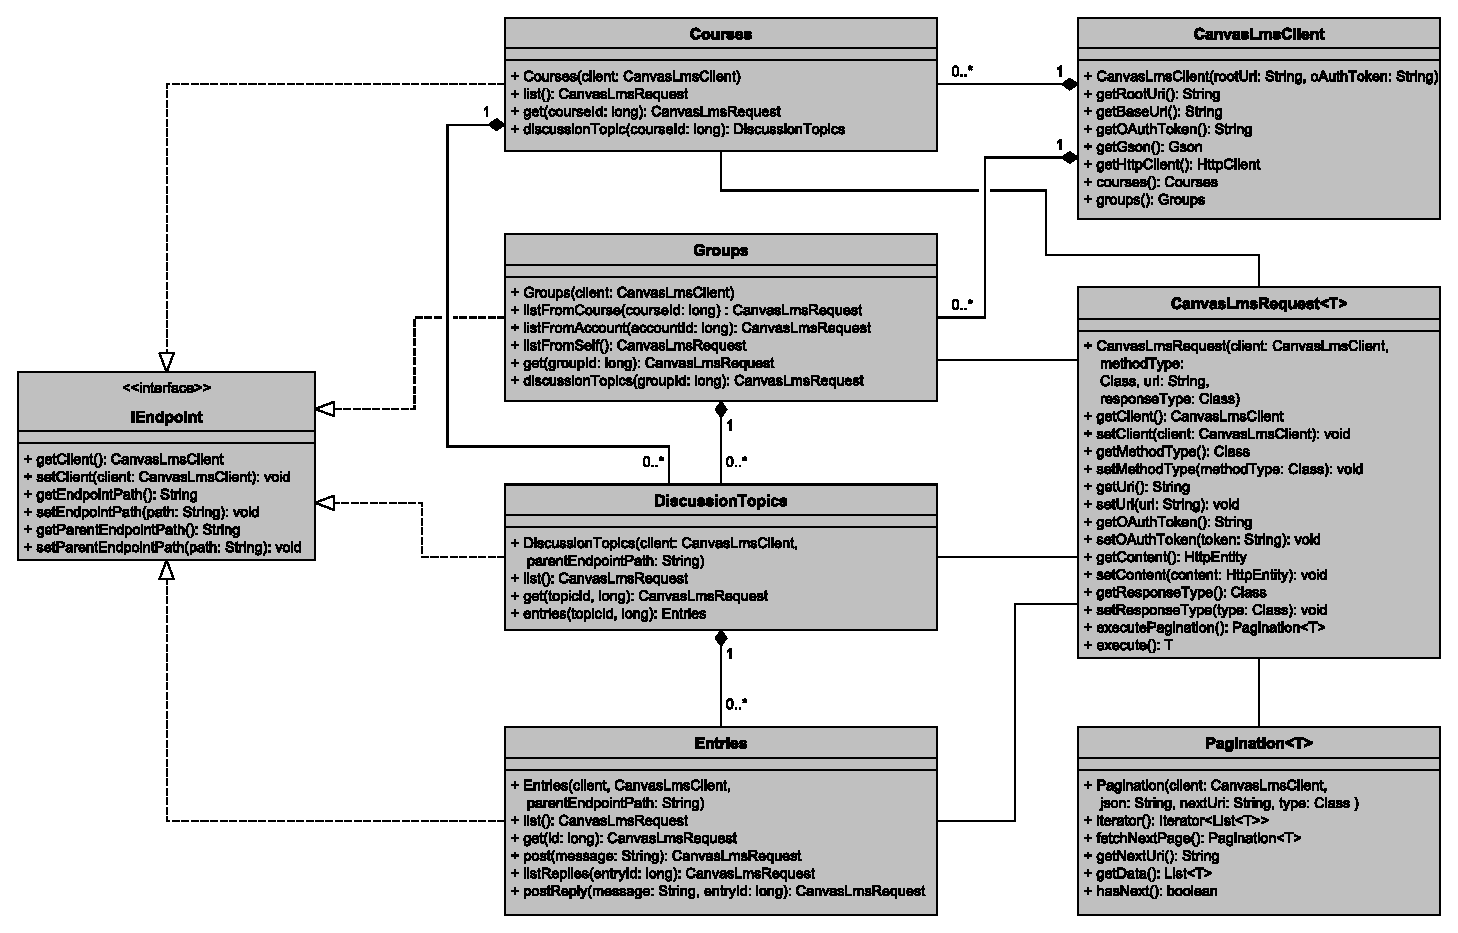
\includegraphics[
        width=\textwidth,
        keepaspectratio=true,]
    {assets/images/canvaslms4j_uml_classdiagramm}
    \caption{UML Klassendiagramm von CanvasLMS4J}
    \label{fig:canvaslms4j_uml_classdiagram}
\end{figure} 

Ausgangspunkt für CanvasLMS4J ist die Klasse \texttt{CanvasLmsClient} (siehe Abbildung \ref{fig:canvaslms4j_uml_classdiagram}). Über sie werden alle Endpunkte verwaltet die keinen Eltern-Endpunkt besitzen. Bei der Erzeugung eines Objektes dieser Klasse, werden ihr die URI zur verwendenden Canvasinstanz und der AccessToken des Benutzerkontos übergeben. Im aktuellen Stadium können von einem Client aus nur Endpunkte für Kurse oder Gruppe erstellt werden.

Endpunkte können dann über die Klasse \texttt{CanvasLmsRequest} REST-Anfragen an die Canvas API stellen. Hierzu verwendet CanvasLMS4J die \emph{HttpClient}\footnote{\url{http://hc.apache.org/httpclient-3.x/}} Bibliothek von Apache mit die einzelnen HTTP-Operationen ausgeführt werden. Um die im JSON-Format zurück gelieferten Antworten der Canvas API in Java verwenden zu können, wir auf die Funktionen der von Google entwickelten \emph{Gson}\footnote{\url{https://code.google.com/p/google-gson/}} Bibliothek zurück gegriffen. Sie erlaubt es Java Objekte in das JSON-Format zu konvertieren und genauso aus Daten in JSON ein Java Objekt zu machen. Dadurch verringert sich der Aufwand für das Verarbeiten der Daten von Canvas auf das Erstellen der entsprechenden Java Klassen. CanvasLmsRequest können mit zwei verschiedenen Methoden ausgeführt werden. Die erste \texttt{execute()} wird dazu verwendet, wenn die REST-Abfrage nur die Rückgabe eines Objektes zu Folge hat. Also zum Beispiel, wenn nur die Daten eines bestimmten Kurses abgefragt werden soll. Die zweite Methode ist \texttt{executePagination}. Diese Methode dient für Abfragen die eine in Seiten aufgeteilte Liste von Ergebnissen zurückliefert und gibt für eine einfache Handhabbarkeit ein Objekt der Klasse \texttt{Pagination} zurück. 

Die Klasse Pagination ist nach dem Iterator Muster aufgebaut und liefert vom kompletten Ergebnis bei jedem Iterationsschritt eine Seite zurück. Diese Seite enthält dann je eine Teilliste der angefragten Objekten. Ist eine Seite fertig ausgelesen, holt Pagination über eine vorgegeben REST Abfrage die nächste Seite. Dies geschieht solange bis keine Seiten mehr geladen werden können oder das Programm das Lesen abbricht.

\begin{lstlisting}[
    caption={CanvasLMS4J Beispielprogramm}\label{lst:canvaslms4j_beispiel},
    captionpos=t]
CanvasLmsClient client = new CanvasLmsClient(
                "https://canvas.instructure.com",
                "7~LUpV7B3lJY...");

Pagination<DiscussionTopic> discussionPages = client.courses()
    .discussionTopics( 798152 )
    .list()
    .executePagination();


for ( List<DiscussionTopic> discussions : discussionPages ) {
    for ( DiscussionTopic discussion : discussions ) {
        System.out.println( discussion );
    }
}

\end{lstlisting}

In Listing \ref{lst:canvaslms4j_beispiel} ist ein Beispiel für die Anwendung der CanvasLMS4J API zu sehen. In den ersten drei Zeilen wird eine neuer CanvasLmsClient für die Canvasinstanz auf \texttt{https://canvas.instructure.com} und einem AccessToken erstellt. Als nächstes soll für einen Kurs mit der ID \enquote{798152} alle Diskussionen aufgelistet werden. Mit dem Aufruf der Methode \texttt{courses()} des Clients wir der Endpunkt für die Kurse und von diesem aus der Endpunkt für die Diskussionen im Kurs \enquote{798152} über die Methode \texttt{.discussionTopics( 798152 )}. In der siebten Zeile wird die Art der Abfrage genauer festgelegt. Da eine Liste alle Diskussionen gesucht ist, wird die Methode \texttt{list()} aufgerufen die ein CanvasLmsRequest Objekt für die gewünschte Abfrage erstellt. Da die Antwort aus mehrere Objekten mit der Beschreibung der einzelnen Diskussionen besteht, wird die Anfrage in Zeile Acht mit der Methode \texttt{executePagination()} ausgeführt. Die einzelnen Seiten des Ergebnisses werden dann in der elften Zeile mit einer For-Schleife durchlaufen. Das nachladen der Seiten erfolgt dabei automatisch durch die Pagination Klasse. Jede Seite besteht nun aus einer Liste mit den Beschreibung der Diskussionen in einem \texttt{DiskussionTopic} Objekt, welche dann wieder in einer weiteren Schleife ausgegeben werden.

% subsubsection canvaslms4j (end)

\subsubsection{Canvas Mapping nach SIOC} % (fold)
\label{ssub:canvas_sioc_mapping}

\begin{table}[ht]
    \centering
    \begin{tabular}{l|p{11cm}}
        \textbf{SIOC Klasse} & \textbf{URI-Format} \\ 
        \hline
        Site & \\
        Service & \\
        UserAccount & \\
        Forum & \\
        Thread & \\
        Post & \\
    \end{tabular}
\end{table}

\begin{table}[ht]
    \centering
    \caption{Format der URIs für Canvas}
    \begin{tabular}{l|p{11cm}}
        \textbf{URI Platzhalter} & URI-Format \\ 
        \hline
        \texttt{\{serviceUri\}} & 
        \texttt{\{rootUri\}/api/v1} \\

        \texttt{\{userAccountUri\}} & 
        \texttt{\{rootUri\}/about/\{userId\}} \\

        \texttt{\{siteUri\}} & 
        \texttt{\{rootUri\}} \\

        \texttt{\{forumUri\}} & 
        \texttt{\{rootUri\}/courses/\{courseId\}},
        \texttt{\{rootUri\}/groups/\{groupId\}} \\

        \texttt{\{threadUri\}} & 
        \texttt{\{forumUri\}/discussion\_topics/\{topicId\}} \\

        \texttt{\{postUri\}} & 
        \texttt{\{threadUri\}/entries/\{entryId\}},
        \texttt{\{threadUri\}\#discussion\_topic} \\
    \end{tabular}
    \label{tbl:canvas_uri_platzhalter}
\end{table}

% subsubsection canvas_sioc_mapping (end)

% subsection canvas_connector (end)

% section implementierung_einiger_connectoren (end)

\section{Evaluation} % (fold)
\label{sec:evaluation}

% section evaluation (end)

% chapter implementierung_und_evaluation (end)